%%%%%%%%%%%%%%%%%%%%%%%%%%%%%%%%%%%%%%%%%%%%%%%%%%%%%%%%%%%%%%%%%%%%%%
% Lớp 10 | Véctơ (chưa xét tọa độ) | Tích của một số với véctơ
% Dạng 0H5?3-8: Cực trị hình học
%%%%%%%%%%%%%%%%%%%%%%%%%%%%%%%%%%%%%%%%%%%%%%%%%%%%%%%%%%%%%%%%%%%%%%


% nguồn: TuLuan_Lop10_Dot2 (nhập 14/11/2026)
\begin{bt}%[0H5H3-8]%[Dự án đề kiểm tra HKI NH22-23 - Quan Ón]%[THPT LƯƠNG NGỌC QUYẾN - THÁI NGUYÊN]%[ma:8310fd10]
	Cho tam giác $ABC$ và đường thẳng $d$.
	\begin{enumerate}
		\item Tìm điểm $I$ để $\overrightarrow{IA} + \overrightarrow{IB} + 3\overrightarrow{IC} = \overrightarrow{0}$.
		\item Tìm trên $d$ điểm $M$ sao cho $\left|\overrightarrow{MA} + \overrightarrow{MB} + 3\overrightarrow{MC} \right| $ nhỏ nhất.
	\end{enumerate}
	\loigiai{
		\begin{center}
			\begin{tikzpicture}[>=stealth,line join=round,line cap=round,font=\footnotesize,scale=0.8]
				\path 
				(1.8,4) coordinate (A)
				(0,2) coordinate (B)
				(4.5,1) coordinate (C)
				(-0.5,0) coordinate (d1)
				(7,0) coordinate (d)
				($(A)!0.5!(B)$) coordinate (E)
				($(E)!1/5!(C)$) coordinate (I1)
				($(E)!2/5!(C)$) coordinate (I2)
				($(E)!3/5!(C)$) coordinate (I)
				($(E)!4/5!(C)$) coordinate (I3)
				($(d1)!(I)!(d)$) coordinate (M);
				\draw[color=gray] (A)--(B)--(C)--(A) (E)--(C) (I)--(M) (d1)--(d);
				\foreach \l/\g in {A/90,B/-135,C/-45,I/60,M/-90,E/120}
				\draw[fill=black] (\l) circle (1pt) +(\g:.3) node{$\l$};
				\draw (d) node[above]{$d$};
				\fill (I1) circle (1pt);
				\fill (I2) circle (1pt);
				\fill (I3) circle (1pt);
				\draw pic[draw,angle radius=1.5mm]{right angle=d--M--I};
			\end{tikzpicture}
		\end{center}
		\begin{enumerate}
			\item Gọi $E$ là trung điểm của $AB$. Ta có $\overrightarrow{IA} + \overrightarrow{IB} = 2\overrightarrow{IE}$ nên
			$$ \overrightarrow{IA} + \overrightarrow{IB} + 3\overrightarrow{IC} = \overrightarrow{0} \Leftrightarrow 2\overrightarrow{IE} = -3\overrightarrow{IC} \Leftrightarrow \overrightarrow{IE} = \dfrac{3}{2}\overrightarrow{IC}. $$
			Vậy $I$ nằm trong đoạn $EC$ sao cho $IE = \dfrac{3}{2}IC$.
			\item Theo ý a) ta có $\overrightarrow{IA} + \overrightarrow{IB} + 3\overrightarrow{IC} = \overrightarrow{0}$.\\
			Khi đó, với mọi điểm $M$ thì
			\begin{eqnarray*}
				\left| \overrightarrow{MA} + \overrightarrow{MB} + 3\overrightarrow{MC} \right| &=& \left| \overrightarrow{MI} + \overrightarrow{IA} + \overrightarrow{MI} + \overrightarrow{IB} + 3\left( \overrightarrow{MI} + \overrightarrow{IC}\right)\right| \\
				&=& \left| 5\overrightarrow{MI}\right| \\
				&=& 5MI.
			\end{eqnarray*}
			Suy ra $\left| \overrightarrow{MA} + \overrightarrow{MB} + 3\overrightarrow{MC} \right|$ nhỏ nhất khi $MI$ nhỏ nhất.\\
			Vậy $M$ là hình chiếu vuông góc của $I$ trên $d$.
		\end{enumerate}
	}
\end{bt}

% nguồn: TuLuan_Lop10_Dot2 (nhập 14/11/2026)
\begin{bt}%[0H5C3-8] % KIEM_TRA%%[ma:740c48b2]
	Cho hình vuông $ABCD$ cạnh $a$, $d$ là đường thẳng  qua $A$, song song với $BD$. Gọi $M$ là điểm
	thuộc đường thẳng $d$ sao cho $|\vec{MA} +\vec{MB} +\vec{MC} -\vec{MD}|$ nhỏ nhất.
	Tính theo $a$ độ dài véc-tơ $\vec{MD}$.
	\loigiai{
		\begin{center}
			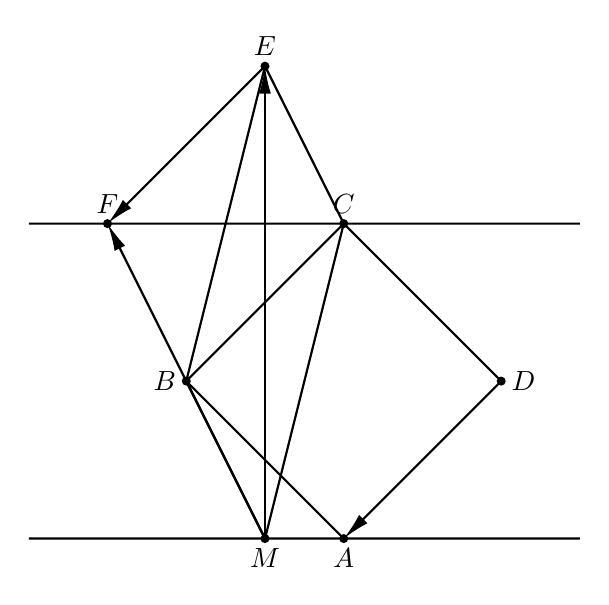
\begin{tikzpicture}[thick]
				\usetikzlibrary{arrows.meta}
				\tikzset{>={Latex[width=1.5mm,length=3.5mm]}}
				\coordinate (A) at (1,0); \coordinate (B) at (-1,2); \coordinate (C) at (1,4);
				\coordinate (D) at (3,2); \coordinate (M) at (0,0);  \coordinate (E) at (0,6);
				\coordinate (F) at (-2,4);
				\draw (A)--(B)--(C)--(D)  (M)--(B)--(E)--(C)--cycle  (-3,0)--(4,0) (-3,4)--(4,4);
				\draw[->] (M)--(F); \draw[->] (M)--(E); \draw[->] (D)--(A);  \draw[->] (E)--(F);
				\foreach \i in {M,A} \draw[fill] (\i) circle (1.2pt) node[below] {$\i$} ;
				\foreach \i in {C,E,F} \draw[fill] (\i) circle (1.2pt) node[above] {$\i$} ;
				\draw[fill] (B) circle (1.2pt) node[left] {$B$} ;
				\draw[fill] (D) circle (1.2pt) node[right] {$D$} ;
			\end{tikzpicture}
		\end{center}
		Dựng hình bình hành $MBEC$, $BCEF$,  ta có $|\vec{MA} +\vec{MB} +\vec{MC} -\vec{MD}| = |\vec{ME} +\vec{DA}| = |\vec{ME} +\vec{EF}| =|\vec{MF}|$. Khi $M$ thay đổi trên $d$ thì $F$ thuộc đường thẳng cố định
		qua $C$ song  song với $d$, điểm $M$ cần tìm là hình chiếu vuông góc của $B$ trên $d$. $|\vec{MD}| =\dfrac{a\sqrt{10}}{2}$.
	}
\end{bt}
